% =====================================================================
% SPEAR-Net architecture figure (TikZ, vector).
% Standalone: `pdflatex architecture.tex`  ->  architecture.pdf
% In the paper: \includegraphics[width=\textwidth]{architecture} (via \graphicspath).
%
% Real image slots (drop PNGs beside this file / in paper_figures/, same names):
%   input_patch.png  ndvi.png mndwi.png ndti.png bsi.png  attention.png
%   prediction.png  edge.png
% If a PNG is absent, a labelled placeholder box is drawn so it still compiles.
%
% Technically faithful to the implementation:
%   * skip fusion is CONCATENATION (C), not addition;
%   * each skip is first GATED by the attention (multiply, F'=F(1+alpha A));
%   * the deepest feature (s5) is the UNGATED decoder bottleneck;
%   * decoder widths 128->64->48->32 run coarse (1/16) -> fine (1/2);
%   * a bilinear upsample to 256^2 precedes the two heads;
%   * the compound loss compares predictions against the ground truth.
% =====================================================================
\documentclass[border=8pt]{standalone}
\usepackage[T1]{fontenc}
\usepackage{lmodern}
\usepackage{amsmath}
\usepackage{amssymb}
\usepackage{xcolor}
\usepackage{graphicx}
\usepackage{tikz}
\usetikzlibrary{arrows.meta,positioning,calc,fit,backgrounds}

\definecolor{pisp}{HTML}{009E73}   % green  - spectral-prior lane
\definecolor{dec}{HTML}{0072B2}    % blue   - decoder lane
\definecolor{enc}{HTML}{4D4D4D}    % gray   - encoder lane
\definecolor{gt}{HTML}{7F7F7F}

% image slot with graceful fallback ------------------------------------
\newcommand{\slot}[2]{% #1 = filename base, #2 = side length
  \IfFileExists{#1.png}
    {\includegraphics[width=#2,height=#2]{#1.png}}
    {\parbox[c][#2][c]{#2}{\centering\ttfamily\tiny \detokenize{#1}.png}}}

\begin{document}
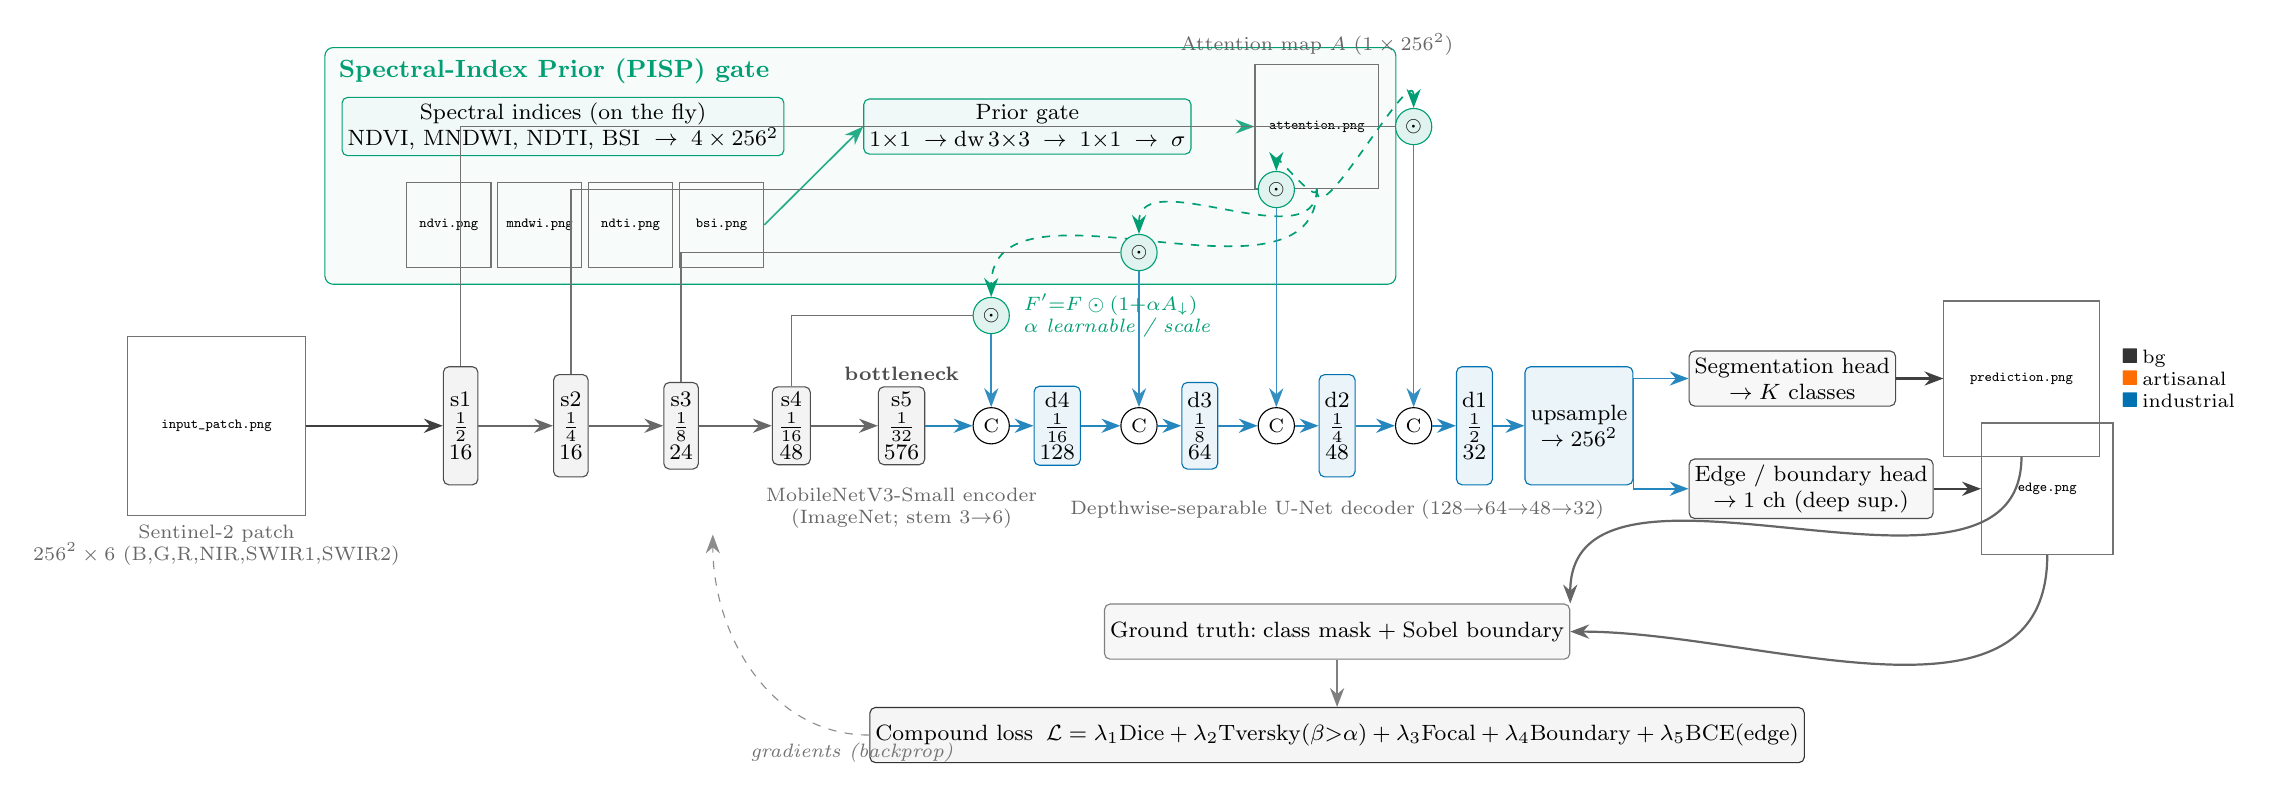
\begin{tikzpicture}[
  >={Stealth[length=2.4mm]},
  font=\footnotesize,
  every node/.style={inner sep=2pt},
  box/.style={rounded corners=2pt,draw,align=center,minimum height=7mm},
  enc/.style={box,draw=enc,fill=enc!7},
  decb/.style={box,draw=dec,fill=dec!8},
  pispb/.style={box,draw=pisp,fill=pisp!6},
  head/.style={box,draw=black!70,fill=black!3,align=center},
  img/.style={draw=black!55,inner sep=1pt},
  op/.style={circle,draw,fill=white,inner sep=0pt,minimum size=4.6mm,font=\scriptsize},
  flow/.style={->,thick,draw=black!75},
  encflow/.style={->,semithick,draw=enc!85},
  decflow/.style={->,semithick,draw=dec!85},
  pispflow/.style={->,semithick,draw=pisp!85},
  attn/.style={->,semithick,draw=pisp,dashed},
  lbl/.style={font=\scriptsize\itshape,text=black!55},
  dim/.style={font=\scriptsize,text=black!60},
]

% ---------------------------------------------------------------- INPUT
\node[img] (in) at (0,0) {\slot{input_patch}{2.2cm}};
\node[dim,below=1pt of in,align=center] {Sentinel-2 patch\\$256^2\times6$ (B,G,R,NIR,SWIR1,SWIR2)};

% ------------------------------------------------ PISP (top green lane)
\node[pispb] (idx) at (4.4,3.8)
  {Spectral indices (on the fly)\\NDVI, MNDWI, NDTI, BSI \;$\to\;4\times256^2$};
\node[img] (t1) at (2.95,2.55) {\slot{ndvi}{1.0cm}};
\node[img,right=2pt of t1] (t2) {\slot{mndwi}{1.0cm}};
\node[img,right=2pt of t2] (t3) {\slot{ndti}{1.0cm}};
\node[img,right=2pt of t3] (t4) {\slot{bsi}{1.0cm}};
\node[pispb,right=10mm of idx,minimum width=26mm] (gate)
  {Prior gate\\$1{\times}1\;\to\;$dw$\,3{\times}3\;\to\;1{\times}1\;\to\;\sigma$};
\node[img,right=8mm of gate] (attnimg) {\slot{attention}{1.5cm}};
\node[dim,above=1pt of attnimg] {Attention map $A$ ($1\times256^2$)};

\draw[pispflow] (t4.east) -- (gate.west);
\draw[pispflow] (gate.east) -- (attnimg.west);

% enclosing PISP panel
\begin{scope}[on background layer]
  \node[draw=pisp,rounded corners=3pt,fill=pisp!3,
        fit=(idx)(t1)(gate)(attnimg),inner sep=6pt] (pisppanel) {};
\end{scope}
\node[anchor=north west,text=pisp,font=\small\bfseries]
  at ([xshift=3pt,yshift=-2pt]pisppanel.north west) {Spectral-Index Prior (PISP) gate};

% -------------------------------------------- ENCODER (shrinking, gray)
\def\ey{0}
\node[enc,minimum height=15mm] (e1) at (3.1,\ey) {s1\\$\tfrac12$\\16};
\node[enc,minimum height=13mm] (e2) at (4.5,\ey) {s2\\$\tfrac14$\\16};
\node[enc,minimum height=11mm] (e3) at (5.9,\ey) {s3\\$\tfrac18$\\24};
\node[enc,minimum height=9mm]  (e4) at (7.3,\ey) {s4\\$\tfrac1{16}$\\48};
\node[enc,minimum height=7mm]  (b)  at (8.7,\ey) {s5\\$\tfrac1{32}$\\576};
\node[dim,below=6pt of b,align=center] (enccap) {MobileNetV3-Small encoder\\(ImageNet; stem $3{\to}6$)};

\draw[flow] (in.east) -- (e1.west);
\draw[encflow] (e1)--(e2); \draw[encflow] (e2)--(e3);
\draw[encflow] (e3)--(e4); \draw[encflow] (e4)--(b);
\node[dim,above=0pt of b,font=\scriptsize\bfseries,text=enc] {bottleneck};

% -------------------------------------------- DECODER (growing, blue)
\node[op,right=6mm of b] (c4) {\scriptsize C};
\node[decb,minimum height=9mm,right=3mm of c4]  (d4) {d4\\$\tfrac1{16}$\\128};
\node[op,right=5mm of d4] (c3) {\scriptsize C};
\node[decb,minimum height=11mm,right=3mm of c3] (d3) {d3\\$\tfrac18$\\64};
\node[op,right=5mm of d3] (c2) {\scriptsize C};
\node[decb,minimum height=13mm,right=3mm of c2] (d2) {d2\\$\tfrac14$\\48};
\node[op,right=5mm of d2] (c1) {\scriptsize C};
\node[decb,minimum height=15mm,right=3mm of c1] (d1) {d1\\$\tfrac12$\\32};
\node[decb,right=4mm of d1,minimum height=15mm,align=center] (up) {upsample\\$\to 256^2$};

\draw[decflow] (b.east) -- (c4);
\draw[decflow] (c4) -- (d4);
\draw[decflow] (d4) -- (c3); \draw[decflow] (c3) -- (d3);
\draw[decflow] (d3) -- (c2); \draw[decflow] (c2) -- (d2);
\draw[decflow] (d2) -- (c1); \draw[decflow] (c1) -- (d1);
\draw[decflow] (d1) -- (up);
\node[dim,below=6pt of d2,align=center]
  {Depthwise-separable U-Net decoder\;(128$\to$64$\to$48$\to$32)};

% -------------------- gated skips: e_k --(gate * )-- C_k, attention -> gate
\foreach \e/\c/\gy/\name in {e4/c4/1.4/g4, e3/c3/2.2/g3, e2/c2/3.0/g2, e1/c1/3.8/g1}{
  \node[op,draw=pisp,fill=pisp!12] (\name) at ($(\c)+(0,\gy)$) {\scriptsize$\odot$};
  \draw[semithick,draw=enc!80] (\e.north) |- (\name.west);
  \draw[semithick,draw=dec!80,->] (\name) -- (\c);
  \draw[attn] (attnimg.south) to[out=-90,in=90] (\name.north);
}
\node[lbl,right=1mm of g4,text=pisp,align=left]
  {$F'{=}F\odot(1{+}\alpha A_{\downarrow})$\\$\alpha$ learnable / scale};

% ------------------------------------------------------- HEADS + OUTPUT
\node[head,right=7mm of up,yshift=6mm]  (seg)  {Segmentation head\\$\to K$ classes};
\node[head,right=7mm of up,yshift=-8mm] (edge) {Edge / boundary head\\$\to 1$ ch (deep sup.)};
\draw[decflow] (up.east) |- (seg.west);
\draw[decflow] (up.east) |- (edge.west);

\node[img,right=6mm of seg]  (pred) {\slot{prediction}{1.9cm}};
\node[img,right=6mm of edge] (edg)  {\slot{edge}{1.6cm}};
\draw[flow] (seg) -- (pred);
\draw[flow] (edge) -- (edg);
\node[anchor=west,font=\scriptsize,align=left] at ([xshift=2mm]pred.east)
  {\textcolor{black!80}{$\blacksquare$}\,bg\\ \textcolor{orange!85!red}{$\blacksquare$}\,artisanal\\ \textcolor{dec}{$\blacksquare$}\,industrial};

% -------------------------------------------------------------- LOSS + GT
\node[head,draw=gt,fill=gt!6,below=16mm of d2,minimum width=42mm] (gtbox)
  {Ground truth:\;class mask\;+\;Sobel boundary};
\node[box,draw=black!80,fill=black!4,below=6mm of gtbox,minimum width=0.86\linewidth] (loss)
  {Compound loss\;\;$\mathcal{L}=\lambda_1\mathrm{Dice}+\lambda_2\mathrm{Tversky}(\beta{>}\alpha)
   +\lambda_3\mathrm{Focal}+\lambda_4\mathrm{Boundary}+\lambda_5\mathrm{BCE(edge)}$};

\draw[flow,draw=black!60] (pred.south)  to[out=-90,in=90] (gtbox.north east);
\draw[flow,draw=black!60] (edg.south)   to[out=-90,in=0]  (gtbox.east);
\draw[flow,draw=gt] (gtbox.south) -- (loss.north);
\draw[->,dashed,draw=black!45] (loss.west) to[out=180,in=-90]
  node[pos=0.06,below=1pt,lbl] {gradients (backprop)}
  ([xshift=-6mm]enccap.south west);

\end{tikzpicture}
\end{document}
